% ##################################################################################################################
\section{Munich}
\label{sec:munich}
\hfill \textbf{Author:} Benjamin Kickh\"ofer

% ##################################################################################################################
The MATSim scenario for the Munich metropolitan area was set up during the year 2010.%
%
\footnote{
%
The most detailed descriptions of the scenario can be found in \citet{KickhoeferEtAl_VanoutriveVerhetsel_2013} and \citet{Kickhoefer_PhDThesis_2014}.
%
}
%
The main goal was, and still is, the simulation of local air pollutant and global greenhouse gas emissions, and how their levels change with respect to different policy measures -- on aggregated and spatially disaggregated level. The scenario was therefore used for the development and testing of the \gls{emt} (see Chapter~\ref{ch:emissions}). For an example on where the overall $\mathit{NO_2}$ emissions produced by private cars and freight vehicles are emitted during the whole day, see Figure~\ref{fig:munich:no2emissions}.

\createfigure%
{$\mathit{NO_2}$ emissions in Munich}%
{$\mathit{NO_2}$ emissions in Munich}%
{\label{fig:munich:no2emissions}}%
{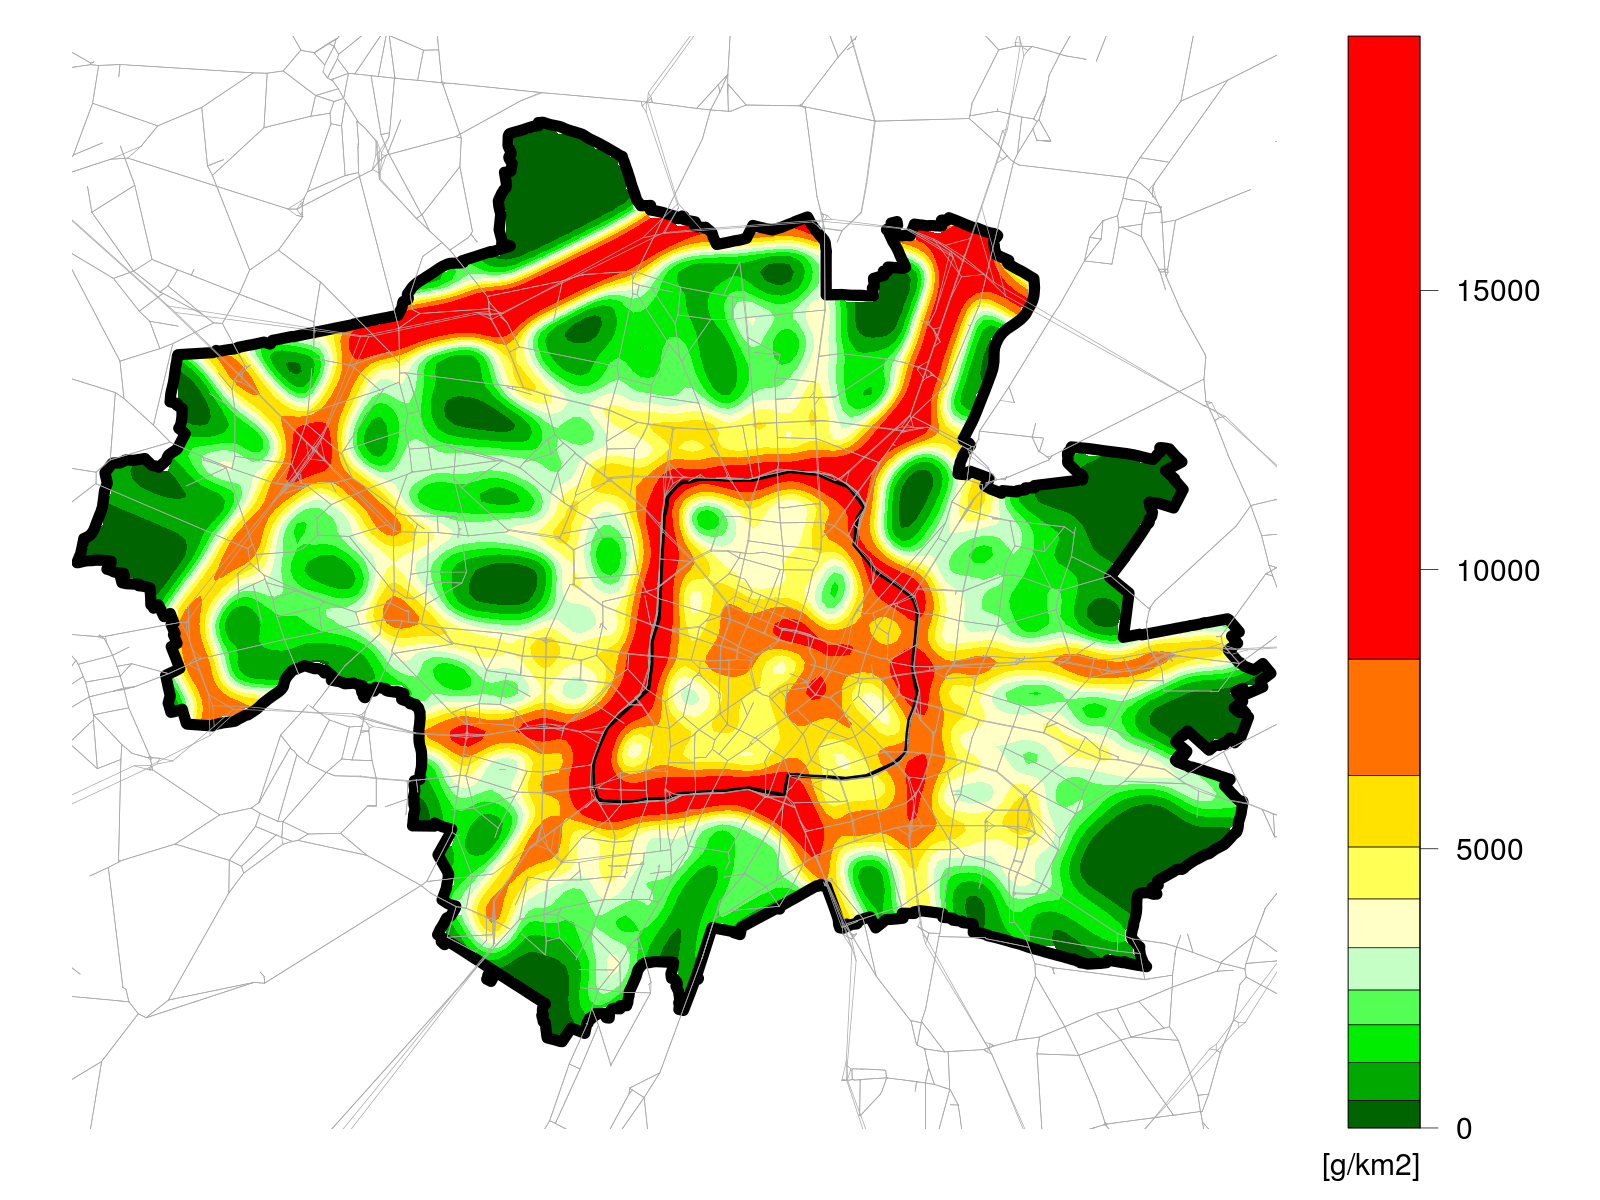
\includegraphics[width=0.85\textwidth, angle=0]{./using/figures/baseCase_1500_NO2_g_108000_0.png}}%
{}

Network information from \acrshort{visum} was converted into MATSim format, resulting in a network of 17\,888 nodes and 41\,942 links.
%
This transport supply was then linked to travel demand from different sources: an activity-based demand for inner-urban traffic from survey data was created based on "Mobility in Germany" \citep[MiD 2002,][]{FollmerEtAl_TechRep_infasDIW_2004}. This part of the synthetic population consists of roughly 1.4\,million individuals with detailed vehicle information for every household.
%
Commuter and reverse commuter were modeled based on data provided by the German Federal Employment Office \citep{BoehmeEigenhueller_TechRep_IAB_2006}. This part of the population consists of roughly 0.5\,million individuals from which 0.3\,million commute to Munich for work. The remaining individuals live in Munich and commute to their workplace in the surroundings of Munich.
%
Freight traffic was also introduced into the model by using data from the German Ministry for Transport \citep{ITBBVU_TechRep_2007}. This part of the population consists of roughly 0.15\,million freight vehicles performing one single commercial trip per day.

The scenario has so far been used for several case studies:
%
\citet{HuelsmannEtAl_LAS_2011} used a single street corridor of the scenario to validate simulated travel times and emission levels against actual data obtained from a test vehicle.
%
\citet{KickhoeferEtAl_VanoutriveVerhetsel_2013} investigate the relationship between the price elasticities of car travel demand and those of air pollutant emissions.
%
\citet{HuelsmannEtAl_GerikeEtAl_2013} identify areas with high air pollution concentration in the city. They define these areas as 'hotspots' since the \gls{eu} limits for \gls{no2} are exceeded. The authors then incrementally raise the toll levels for passing the hotspots until they disappear in order to estimate the true avoidance costs of the \gls{eu} threshold values.
%
\citet{KickhoeferEtAl_NSE_2013} derive time-dependent vehicle-specific first-best air pollution tolls in order to create a benchmark for the evaluation of real-world policies.
%
\citet{KickhoeferKern_MobilTUM_2014} go a step beyond and calculate time-dependent vehicle-specific air pollution exposure tolls in order to correct the toll levels by \citet{KickhoeferEtAl_NSE_2013} for the number of affected individuals.



% ##################################################################################################################